\documentclass[a4paper,11pt]{article}
\usepackage[utf8]{inputenc}
\usepackage[english]{babel}
\usepackage[colorlinks=true, urlcolor=black, linkcolor=black]{hyperref}
\usepackage[margin=3cm]{geometry}
\usepackage{parskip}
\usepackage{hyperref}
\usepackage{graphicx}

\setlength{\parindent}{3em}

\author{
	\Large Cerezo Pomykol, Jan\\ \href{mailto:j.cerezo@alumnos.upm.es}{\small\texttt{j.cerezo@alumnos.upm.es}}
}

\title{\textbf{\Huge Practical Application 1} \\
		\Large Machine Learning}

\date{\Large October 18, 2022}

\begin{document}
\maketitle
\vfill

\tableofcontents
\newpage

\section{Introduction}
\label{sec:introduction}

The goal of this practical application is to study how feature subset selection (FSS) affects different machine learning models. Specifically how they perform with a dataset with all variables and datasets obtained from a univariate filter, a multivariate filter, and a multivariate wrapper. The selected classification models are the following:

\begin{itemize}
\item k-Nearest Neighbours.
\item Rule Induction - RIPPER algorithm.
\item Support Vector Machines.
\item Neural Network - Multilayer Perceptron.
\item Classification Trees - C4.5 algorithm.
\end{itemize}

For this assignment, the dataset chosen \cite{misc_dry_bean_dataset_602}\cite{KOKLU2020105507} contains data about instances of dry beans, which was created from images of 13,611 grains of 7 different varieties.

The rest of the document has the following structure. Firstly, de dataset is analysed in the \hyperref[sec:problem]{Problem Description}, later the methodology is specified in the \hyperref[sec:methodology]{Methodology section}. Subsequently the results are shown in the \hyperref[sec:results]{Results section}, and finally they are analysed in the \hyperref[sec:discussion]{Discussion} and \hyperref[sec:conclusion]{Conclusion} sections.

\section{Problem Description}
\label{sec:problem}

The dataset contains 13,611 instances created from images of dry beans of 7 different varieties. There are a total of 17 attributes (16 plus the class column) and their significance is the following:

\begin{itemize}
\setlength\itemsep{-1ex}
\item[1] \textbf{Area} (A): The area of a bean zone and the number of pixels within its boundaries.
\item[2] \textbf{Perimeter} (P): Length of its border.
\item[3] \textbf{Major axis length} (L): Length of the longest line that can be drawn from a bean.
\item[4] \textbf{Minor axis length} (l): Length of the longest line that can be drawn from the bean while standing perpendicular to the main axis.
\item[5] \textbf{Aspect ratio} (K): Relationship between L and l.
\item[6] \textbf{Eccentricity} (Ec): Eccentricity of the ellipse having the same moments as the region.
\item[7] \textbf{Convex area} (C): Number of pixels in the smallest convex polygon that can contain the area of a bean seed.
\item[8] \textbf{Equivalent diameter} (Ed): The diameter of a circle having the same area as a bean seed area.
\item[9] \textbf{Extent} (Ex): The ratio of the pixels in the bounding box to the bean area.
\item[10] \textbf{Solidity} (S): Also known as convexity. The ratio of the pixels in the convex shell to those found in beans.
\item[11] \textbf{Roundness} (R): Calculated with the following formula: $\frac{4\pi A}{P^2}$
\item[12] \textbf{Compactness} (CO): Measures the roundness of an object: $\frac{Ed}{L}$
\item[13] \textbf{ShapeFactor1} (SF1)
\item[14] \textbf{ShapeFactor2} (SF2)
\item[15] \textbf{ShapeFactor3} (SF3)
\item[16] \textbf{ShapeFactor4} (SF4)
\item[17] \textbf{Class}: Seker, Barbunya, Bombay, Cali, Dermosan, Horoz and Sira.
\end{itemize}

All attributes are numeric, except the class which is nominal. Additionally, there are no \textit{meta-attributes} such as instance or object identifiers, so there is no need to remove any column. \autoref{tab:table1} shows more information about the ranges of values and \autoref{tab:table2} shows the number of instances of each class.

\begin{table}[h]
\centering
\begin{tabular}{||l|l|l|l||}
	\hline
	No. & Name & Min. & Max.\\
	\hline
	1 & Area & 20420 & 254616\\
	2 & Perimeter & 524.736 & 1985.37\\
	3 & Major axis length & 183.601 & 738.86\\
	4 & Minor axis length & 122.513 & 460.198\\
	5 & Aspect ratio & 1.025 & 2.43\\
	6 & Eccentricity & 0.219 & 0.911\\
	7 & Convex area & 20684 & 263261\\
	8 & Equivalent diameter & 161.244 & 569.374\\
	9 & Extent & 0.555 & 0.866\\
	10 & Solidity & 0.919 & 0.995\\
	11 & Roundness & 0.49 & 0.991\\
	12 & Compactness & 0.641 & 0.987\\
	13 & ShapeFactor1 & 0.003 & 0.01\\
	14 & ShapeFactor2 & 0.001 & 0.004\\
	15 & ShapeFactor3 & 0.41 & 0.975\\
	16 & ShapeFactor4 & 0.948 & 1\\
	17 & Class & - & -\\
	\hline
\end{tabular}
\caption{Value ranges of each variable.}
\label{tab:table1}
\end{table}

\begin{table}[h]
\centering
\begin{tabular}{||l|l||}
	\hline
	Class & n\\
	\hline
	SEKER & 2027\\
	BARBUNYA & 1322\\
	BOMBAY & 522\\
	CALI & 1630\\
	HOROZ & 1928\\
	SIRA & 2636\\
	DERMASON & 3546\\
	\hline
\end{tabular}
\caption{Number of instances per class.}
\label{tab:table2}
\end{table}

Since there are some variables with high values compared to others (for example Area compared to Extent); normalization is necessary.

\section{Methodology}
\label{sec:methodology}

\subsection{Software}
\label{subsec:software}

For this practical application, Weka \cite{weka} has been used to perform the training and evaluation of all models, as well as the normalization of the dataset. Besides from normalization of the dataset, there is no need to perform more pre-processing. There are no missing values and all variables are numerical (except the class).

\subsection{Evaluation}
\label{subsec:evaluation}

The evaluation of each model will be conducted with cross validation with 10 folds. Because each class has different weight (different number of instances) the confusion matrix will be discussed as well. Besides the accuracy, training time will also be considered.

\subsection{Classification Algorithms}
\label{subsec:algorithms}

The following machine learning algorithms have been evaluated. Note that some of them have the option to normalize de input data, which was set to \textit{false} because the data was already normalized in the pre-processing stage.

\begin{itemize}
\item \textbf{k-Nearest Neighbour}. The parameter \textit{k} was set to 10 neighbours.
\item \textbf{Rule Induction}. For this classification method the RIPPER algorithm was used.
\item \textbf{Support Vector Machine}. Non-linear with a polynomial kernel of exponent 2, since it can fit more complex distributions.
\item \textbf{Neural Network}. With \textit{t} neurons (\textit{t} = attributes + classes) and a single hidden layer.
\item \textbf{Classification Tree}. C4.5 algorithm. This algorithm is an improved version of the ID3 algorithm that uses a gain ratio to choose attributes. It also penalizes attributes with many values and many uniformly distributed values.
\end{itemize}

\autoref{tab:table3} shows the Weka function associated to each algorithm.

\begin{table}[h]
\centering
\begin{tabular}{||l|l||}
	\hline
	Algorithm & Weka Function\\
	\hline
	k-Nearest Neighbours & lazy.IBk\\
	Rule Induction (RIPPER) & rules.JRip\\
	Support Vector Machine & functions.SMO\\
	Neural Network & functions.MultilayerPerceptron\\
	Classification Tree (C4.5) & trees.J48\\
	\hline
\end{tabular}
\caption{Weka implementation of each algorithm.}
\label{tab:table3}
\end{table}

\subsection{Feature Subset Selection}
\label{subsec:fss}

The selection of features has been performed with the following algorithms. \autoref{tab:table4} shows the Weka function associated to each method.

\begin{itemize}
\setlength\itemsep{-1ex}
\item \textbf{No FSS}. The original dataset was used.
\item \textbf{Univariant Filter}. Evaluates the worth of each attribute by measuring the information gain with respect to the class. The threshold used for this dataset is 1.2.
\item \textbf{Multivariant Filter}. Evaluates the worth of a subset of attributes by considering the individual predictive ability of each feature along with the degree of redundancy between them.
\item \textbf{Wrapper Approach}. Evaluates each subset of attributes with the estimated performance of a classifier built with this subset of attributes.
\end{itemize}

\begin{table}[h]
\centering
\begin{tabular}{||l|l||}
	\hline
	FSS algorithm & Weka Function\\
	\hline
	No FSS & -\\
	Univariant Filter & attributeSelection.InfoGainAttributeEval\\
	Multivariant Filter & attributeSelection.CfsSubsetEval\\
	Wrapper Approach & attributeSelection.WrapperSubsetEval\\
	\hline
\end{tabular}
\caption{Weka implementation of each FSS algorithm.}
\label{tab:table4}
\end{table}

Note that the optimization of each classification model and feature selection method is not part of this practical application.

\section{Results}
\label{sec:results}

This section includes the scores obtained with each classifier (\hyperref[subsec:algorithms]{section 3.3}) and each Feature Subset Selection approach (\hyperref[subsec:fss]{section 3.4}). \autoref{tab:table5} shows the attributes selected by each method.

\begin{table}[h]
\centering
\begin{tabular}{||l|c|c|c|c|c|c|c|c||}
	\hline
	Attribute & \rotatebox[origin=c]{90}{No FSS} & \rotatebox[origin=c]{90}{Univariant} & \rotatebox[origin=c]{90}{Multivariant} & \rotatebox[origin=c]{90}{Wrapper (RIPPER)} & \rotatebox[origin=c]{90}{Wrapper (kNN k=7)} & \rotatebox[origin=c]{90}{Wrapper (SVM)} & \rotatebox[origin=c]{90}{Wrapper (MLP)} & \rotatebox[origin=c]{90}{Wrapper (C4.5)}\\
	\hline
	Area & $\bullet$ & $\bullet$ & & & & & & $\bullet$\\
    Perimeter & $\bullet$ & $\bullet$ & $\bullet$ & $\bullet$ & $\bullet$ & $\bullet$ & $\bullet$ &\\
    MajorAxisLength & $\bullet$ & $\bullet$ & $\bullet$ & & & & &\\
    MinorAxisLength & $\bullet$ & $\bullet$ & $\bullet$ & & $\bullet$ & & $\bullet$ &\\
    AspectRatio & $\bullet$ & & $\bullet$ & & & & $\bullet$ &\\
    Eccentricity & $\bullet$ & & & & & & $\bullet$ &\\
    ConvexArea & $\bullet$ & $\bullet$ & $\bullet$ & & & $\bullet$ & & $\bullet$\\
    EquivDiameter & $\bullet$ & $\bullet$ & & $\bullet$ & & $\bullet$ & & $\bullet$\\
    Extent & $\bullet$ & & $\bullet$ & & & $\bullet$ & $\bullet$ &\\
    Solidity & $\bullet$ & & & $\bullet$ & $\bullet$ & $\bullet$ & $\bullet$ & $\bullet$\\
    Roundness & $\bullet$ & & $\bullet$ & $\bullet$ & $\bullet$ & $\bullet$ & $\bullet$ & $\bullet$\\
    Compactness & $\bullet$ & & $\bullet$ & $\bullet$ & & $\bullet$ & $\bullet$ & $\bullet$\\
    ShapeFactor1 & $\bullet$ & $\bullet$ & $\bullet$ & $\bullet$ & $\bullet$ & $\bullet$ & $\bullet$ &\\
    ShapeFactor2 & $\bullet$ & $\bullet$ & $\bullet$ & & $\bullet$ & & $\bullet$ & $\bullet$\\
    ShapeFactor3 & $\bullet$ & & & $\bullet$ & & & &\\
	ShapeFactor4 & $\bullet$ & & $\bullet$ & $\bullet$ & $\bullet$ & $\bullet$ & $\bullet$ & $\bullet$\\
    \hline
    \textbf{N attributes} & 16 & 8 & 11 & 8 & 7 & 9 & 11 & 8\\
    \hline
\end{tabular}
\caption{Attributes selected with each FSS algorithm.}
\label{tab:table5}
\end{table}

\autoref{tab:table6} shows the score of each classification algorithm with all datasets obtained from each Feature Subset Selection method described, and \autoref{tab:table7} shows the training time of each model. The full version of each result report including the confusion matrices can be found in \cite{repo}.

Note that images of the trees obtained by the C4.5 algorithm, or the neural networks generated are not shown because there are too many nodes to show and the representation is not understandable. All the rules generated from the RIPPER algorithm and the support vectors from the SVMs can be found in the complete result reports. In the same way, a representation of the outputs of the kNN algorithm is not included because it is not possible to visualize a 16-dimensional space.

\begin{table}[h]
\centering
\begin{tabular}{||l|l|l|l|l|l||}
	\hline
	Dataset & kNN & RIPPER & SVM & MLP & C4.5\\
	\hline
	Original & 92.0579 & 91.4775 & 92.5648 & 92.7852 & 91.4995\\
	Univariate Filter & 90.8309 & 90.2432 & 89.9052 & 91.2718 & 90.3681\\
	Multivariate Filter & 92.0432 & 91.1395 & 92.4987 & 92.5428 & 91.0073\\
	Wrapper (kNN) & 92.4914 & 91.5436 & 92.4546 & 92.5648 & 91.382\\
	Wrapper (RIPPER) & 92.5354 & 91.4261 & 92.4106 & 92.4693 & 91.4628\\
	Wrapper (SVM) & 92.315 & 91.4187 & 92.5281 & 92.7044 & 91.3452\\
	Wrapper (MLP) & 92.1608 & 91.4334 & 92.5648 & 92.6971 & 91.3085\\
	Wrapper (C4.5) & 92.3885 & 91.4628 & 92.3297 & 92.4546 & 91.4040\\
    \hline 
\end{tabular}
\caption{Scores of all classifiers with all obtained datasets (percentage of correctly classified instances).}
\label{tab:table6}
\end{table}

\begin{table}[h]
\centering
\begin{tabular}{||l|l|l|l|l|l||}
	\hline
	Dataset & kNN & RIPPER & SVM & MLP & C4.5\\
	\hline
	Original & $<$0.1 & 2.38 & 7.98 & 33.37 & 0.3\\
	Univariate Filter & $<$0.1 & 1.89 & 12.11 & 14.87 & 0.1\\
	Multivariate Filter & $<$0.1 & 2.43 & 6.16 & 20.67 & 0.18\\
	Wrapper (kNN) & $<$0.1 & 2.41 & 6.69 & 13.43 & 0.21\\
	Wrapper (RIPPER) & $<$0.1 & 1.67 & 6.82 & 14.89 & 0.12\\
	Wrapper (SVM) & $<$0.1 & 1.74 & 6.13 & 16.64 & 0.14\\
	Wrapper (MLP) & $<$0.1 & 1.91 & 6.71 & 20.56 & 0.17\\
	Wrapper (C4.5) & $<$0.1 & 1.99 & 6.33 & 15.19 & 0.14\\
    \hline 
\end{tabular}
\caption{Training time in seconds.}
\label{tab:table7}
\end{table}

\section{Discussion}
\label{sec:discussion}

Generally, the models trained obtained a score of at least 90\% in most cases. However, the results do not differ greatly from each other. The greatest precision obtained is 92.7852\%, which was achieved with the original dataset and a Multilayer Perceptron classification algorithm.

Overall, the best performing models are the Multilayer Perceptron, the Support Vector Machine, and the k-Nearest Neighbour. Note that the latter has a training time hundreds of times faster compared to the first two.

Regarding the selection of features of this dataset, it is clear that not all variables are needed to obtain models that perform as well as the model generated from all attributes.

In the case of the k-Nearest Neighbours, the reduced datasets obtained slightly better scores than the original dataset. This is probably due to some moderate overfitting. With the \textit{k} parameter set to 10 the model could not fit all de dataset information, because with 10 clusters it is not possible to separate all the classes. This model obtained the best results when the training time is considered.

The Rule Induction classifier did not perform as well as the k-Nearest Neighbours. It obtained slightly poorer results than the kNN implementation, while spending more computational resources.

Both the Support Vector Machine and the Multilayer Perceptron obtained the best results. This is because both models can fit more complex data distributions than the other methods. The SVM calculated more than 1,200 support vectors for each dataset, while the MLP used between 20 and 29 neurons (\autoref{fig:nn}). The complexity of this models is reflected in the training times, which are significantly higher than the other algorithms.

\begin{figure}[h]
\centering
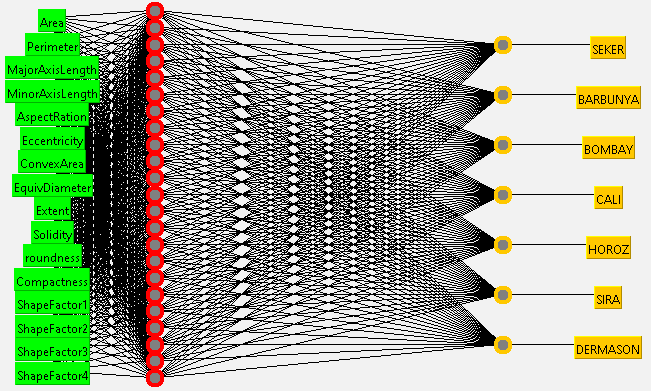
\includegraphics[width=0.85\textwidth]{nn}
\caption{Neural network obtained from the original dataset.}
\label{fig:nn}
\end{figure}

Lastly the tree algorithm performed the same as the RIPPER algorithm, while spending approximately 10 times less computational time to train the models. A representation of the tree is shown in \autoref{fig:tree}. However, it is hardly understandable since Weka does not allow to rescale the size of the graph representation.

\begin{figure}[h]
\centering
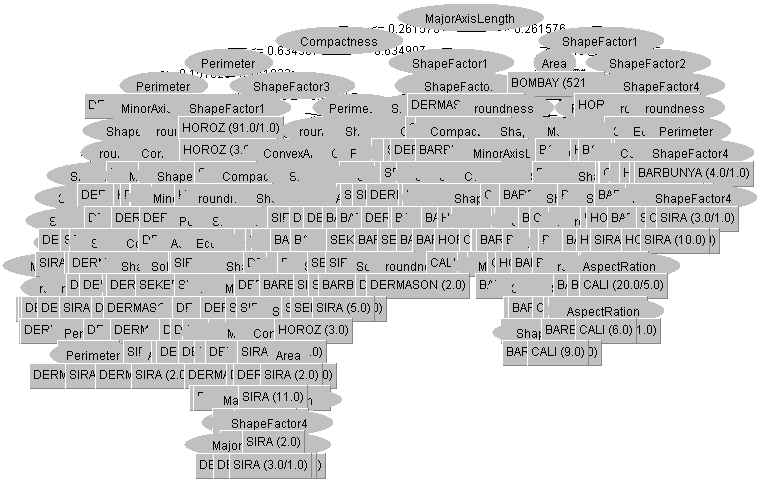
\includegraphics[width=0.9\textwidth]{tree}
\caption{Tree obtained from the original dataset.}
\label{fig:tree}
\end{figure}

Inspecting \autoref{tab:table6} we can deduce that in most cases the reduced datasets obtain similar scores to the original dataset. This is because there are variables that provide no additional information, in other words, there are dependent or irrelevant variables in the dataset. As stated in the \hyperref[sec:problem]{Problem Description section}, there are some variables that are calculated from others. For instance, the \textit{Roundness} is obtained from the \textit{Area} and the \textit{Perimeter}, and the \textit{Compactness} from the \textit{Equivalent diameter} and the \textit{Major axis length}. Additionally, there are some attributes that are fundamentally related, such as the \textit{Area} and the \textit{Perimeter}. The most selected variables are the \textit{Perimeter}, the \textit{Roundness}, and the \textit{Shape Factor 1}.

Looking at \autoref{tab:table5}, both the Univariant Filter and the Wrapper approach with the RIPPER classifier selected 8 features. However, as \autoref{tab:table6} shows, the scores are better in the latter. This means that there are some features selected by the Wrapper that have not been selected by the Univariant Filter that are \textit{significant}. For example, the Wrapper selected \textit{Shape Factor 3 and 4} and \textit{Solidity, Compactness and Roundness}, which were not selected by the Filter. This means that these attributes provide relevant information.

The rest of the reduced datasets obtained similar scores compared to the original dataset. The cause of this is the redundancy of some variables. However, the scores are not close to 100\%, probably because the dataset contains multiple irrelevant attributes, and the isolated \textit{important} features need more complex models to fit the distribution.

\autoref{tab:table8} shows the confusion matrix obtained by the Multilayer Perceptron with the original dataset (the best precision achieved). In this scenario, all instances of the class \textit{BOMBAY} are classified correctly, this is probably due to the fact that the class has a well-defined boundary that could be fitted perfectly by this classification model. In contrast, the other classes had some instances wrongly classified because the algorithm could not fit to the boundaries between each other.

\begin{table}[h]
\centering
\begin{tabular}{||c||c|c|c|c|c|c|c||}
	\hline
	Classified as $\rightarrow$ & a & b & c & d & e & f & g\\
	\hline
	\hline
	a = SEKER & 1929 & 8 & 0 & 0 & 0 & 55 & 35\\
	\hline
	b = BARBUNYA & 10 & 1207 & 0 & 74 & 5 & 25 & 1\\
	\hline
	c = BOMBAY & 0 & 0 & 522 & 0 & 0 & 0 & 0\\
	\hline	
	d = CALI & 3 & 47 & 0 & 1535 & 29 & 16 & 0\\
	\hline
	e = HOROZ & 0 & 3 & 0 & 25 & 1843 & 44 & 13\\
	\hline
	f = SIRA & 31 & 12 & 0 & 7 & 34 & 2291 & 261\\
	\hline
	g = DERMASON & 44 & 1 & 0 & 0 & 8 & 191 & 3302\\
    \hline 
\end{tabular}
\caption{Confusion matrix of the MLP trained with the original dataset.}
\label{tab:table8}
\end{table}

\section{Conclusion}
\label{sec:conclusion}

In this practical application, a dataset of dry beans with 13,611 instances and 17 features (including the class) was analysed with different attribute selection methods and different classifiers with a 10-fold cross-validation test approach. The dataset contains instances of seven different classes. The only pre-processing needed was the normalization of the dataset, since there are no missing values or nominal variables (except the class column).

Different datasets were obtained from the original by extracting features with a Univariate Filter, Multivariate Filter, and different Wrapper approaches. All of which were tested with the following classifiers: k-Nearest Neighbour, RIPPER, Support Vector Machine, Multilayer Perceptron and C4.5.

Overall, the precision obtained is similar in most cases, the best ones obtained by the MLP, SVM, and kNN with the original dataset. Generally, both SVM and MLP obtained better scores than RIPPER and C4.5 due to the ability to fit more complex data distributions. However, the impact of the complexity of the models is reflected in the training time.

The k-Nearest Neighbour classifier performed the best when the execution time is taken into consideration. It obtained better scores than the RIPPER and C4.5 algorithms, while consuming less computational time. Note that the optimization of each model (finding the best combination of hyperparameters) is not part of this assignment, but it could be an interesting subsequent work.

On the other side, in most cases the datasets obtained by selecting features did not obtain better precision than the original dataset. Nevertheless, the reduction of attributes did reduce the training time approximately by half in the Multilayer Perceptron and C4.5 classifiers. Some attributes, for instance the \textit{Perimeter} and the \textit{Roundness} were selected by most feature selection methods, which denotes the importance of these.

In summary, the dataset used in this practical application contains variables that are not needed to achieve similar scores to the original dataset. The best precision was obtained by the Multilayer Perceptron, which can fit more complex data compared to other classification algorithms. However, the k-Nearest Neighbour algorithm achieved similar scores while spending significantly less computational time to train the model.

\newpage
\bibliography{references}
\bibliographystyle{ieeetr}

\end{document}
